\documentclass[11pt]{article}
\usepackage[a4paper]{geometry}
\usepackage{kotex}
\usepackage{hyperref}
\usepackage{subcaption}
\usepackage{caption}
\usepackage{graphicx}
\usepackage{float}
\hypersetup{
    colorlinks,
    citecolor=black,
    filecolor=black,
    linkcolor=black,
    urlcolor=black
}
\usepackage[
    type={CC},
    modifier={by-nc-sa},
    version={3.0},
]{doclicense}

\title{Marina Bay sands tutorial}
\author{채희진}
\date{\today}

\renewcommand{\abstractname}{초록}

\begin{document}
    

\maketitle
\thispagestyle{empty}
\clearpage

\doclicenseThis
\thispagestyle{empty}
\clearpage

\tableofcontents
\thispagestyle{empty}
\clearpage

\pagenumbering{arabic}

\begin{abstract}
   \href{https://www.safdiearchitects.com/projects/marina-bay-sands-integrated-resort}{Marina Bay Sands(MBS)}는 Safdie라는 콧수염난 아저씨가 차린 회사에서 한 프로젝트로, Autodesk University에 MBS 및 Changi 공항 프로젝트가 올라온 바 있습니다. 
   본 노트에서는 Dynamo를 이용해 구성되어 있던 예제를 이해해서 Grasshopper로 만들고, 이 과정에서 필요한 실무적인 지식을 소개합니다. 
\end{abstract}

\section{레이어 관리}
그래스호퍼를 위주로 설명하지만, 실무 상황을 가정하고 몇가지 다른이야기도 섞어서 소개하도록 하겠습니다. 프로젝트를 하면서 가장 중요한 것 중 하나는 레이어 관리입니다.
 가장 좋은 상황은 모든 팀이 정해놓은 따라 레이어를 쓴다면 고생할 일이 없지만, 대부분 상황에서는 레이어 표준이라는 개념이 희박합니다. 또한 건축 특성상 프로젝트별 차이가 있기 때문에
 각 상황에서 문재렬 해결하기 위한 가장 유용한 판단을 내리는 것이 중요합니다.

 레이어 이름을 정할때 Product breakdown structure(PBS)에 따라 하는게 제일 좋습니다. 즉, 건물을 하나의 제품으로 보고, 프로젝트 안에 건물과 대지, 건물 안에 층, 층 안에 벽 등등으로 좁혀 나가는 방식입니다.
 Ghery techonologies(GT)에서도 여기에 기반해 레이어를 만들고 관리를 하고 있는 것으로 알고있고, 특이한점은 꼭 영어 알파벳 3자리를 고집한다는 것입니다. 

 예를 들어, Marina bay sands라면 MBS로 가장 상위 레이어를 정하고, 그아래 DRV(Driver, 핵심 지오메트리), FAC(Facade, 외피), SIT(Site, 대지) 등으로 구분하는 방식입니다(Figure \ref{fig:ghery_example}). 해당 구조를 통해 레이얼르 구성하면 
 MBS-DRV 이런식으로 구성이 가능 합니다. 이렇게 3글자를 기준으로 하면 레이어 이름이 과도하게 늘어나는 것을 방지할 수 있습니다. 하지만 때로는 지나치게 줄여서 어떤의미인지 어려울 때도 있습니다.
 제 개인적인 의견은 3글자인지 4글자인지가 중요한게 아니고, PBS를 적용했다는 것이고 프로그래밍 측면에서 보면 중간에 대시(-)를 일관적으로 넣는 일이 더 중요하다고 생각합니다.
 왜냐하면 프로젝트를 할때 레이어 이름을 이용해서 작업을 하는 경우도 있기 때문입니다.
 \begin{figure}[H]
    \centering
    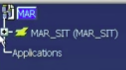
\includegraphics[width=.3\textwidth]{./img/ghery_example}
    \caption[Caption for LOF]{GT에서 사용하는 레이어 관리 방식\footnotemark}
    \label{fig:ghery_example}
 \end{figure}

\footnotetext{\href{https://youtu.be/hr4Vk5lGucU?t=129}{https://youtu.be/hr4Vk5lGucU?t=129}}
다시 돌아와 레이어를 정리해보도록 하겠습니다. 레이어를 정리할때 핵심은 그래스호퍼의 입력값으로 들어갈 값들을 잘 정리하는 것입니다. 본 프로젝트에서는 가장 상위 구조를 MBS로 정했습니다. 그리고 눈으로 확인용으로 쓰는 주변 Geoemtry들은 \textit{MBS-Context}에 포함시켰고,
Grasshopper의 입력값으로 사용될 예정인 값들은 \textit{MBS-Driver}아래에 각각 분리해서 정리했습니다.

\begin{figure}[H]
    \centering
    \begin{subfigure}{.45\textwidth}
        \centering
        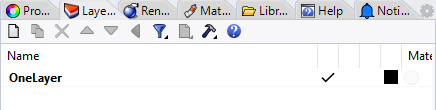
\includegraphics[width=.9\textwidth]{./img/mbs_layer_before}
        \caption{레이어 정리 전}
        \label{fig:1}
    \end{subfigure}
    \begin{subfigure}{.45\textwidth}
        \centering
        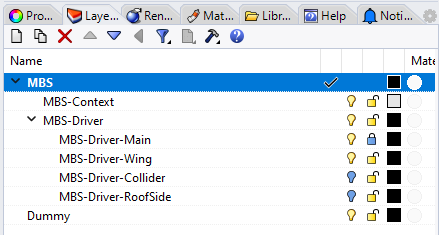
\includegraphics[width=.9\textwidth]{./img/mbs_layer_after}
        \caption{레이어 정리 후}
        \label{fig:2}
    \end{subfigure}
    \caption{레이어 정리 전후 비교}
    \label{fig:layer_before_after}
\end{figure}

\end{document}